\documentclass{presets}
%\documentclass[graybox,envcountchap]{SVMonoEnhanced}
%\usepackage{type1cm}
%\usepackage[utf8]{inputenc}
%%\usepackage[T1]{fontenc}
%\usepackage[russian,english]{babel}
%\usepackage{hyperref}
%\usepackage[table,xcdraw]{xcolor}
%
%\usepackage[none]{hyphenat}
%\usepackage{amssymb,amscd, amsmath, amsfonts, amssymb, newtxtext,newtxmath}
%\usepackage{makeidx, graphicx}
%\usepackage[bottom]{footmisc}
%\usepackage{parskip}
%\usepackage{setspace}
%\usepackage{stackengine}
%\usepackage[margin=2.4cm]{geometry}
%\usepackage{fancyhdr}

%\pagestyle{fancy}
%\renewcommand{\sectionmark}[1]{\markright{\thesection~ #1}}
%\renewcommand{\chaptermark}[1]{\markboth{\thechapter~ #1}{}}
%
%\fancyhead[LO]{\rightmark}
%\fancyhead[RE]{\leftmark}
%\fancyhead[LE,RO]{\thepage}
%\renewcommand{\headrulewidth}{0pt}

%\usepackage{vmargin}
%\setmarginsrb{3 cm}{2.4 cm}{3 cm}{2.4 cm}{1 cm}{1.5 cm}{1 cm}{1.5 cm}



%\renewcommand{\baselinestretch}{1.25}
%\newcommand\xrowht[2][0]{\addstackgap[.5\dimexpr#2\relax]{\vphantom{#1}}}
%\newcommand{\unit}[1]{\ensuremath{\, \mathrm{#1}}}
%
%\graphicspath{{images/}}

\title{Project Report}
\author{Nguyen Quy Khoi}
\date{30 June 2020}

\makeindex
\makeatletter
\let\thetitle\@title
\let\theauthor\@author
\let\thedate\@date
\makeatother
\begin{document}
		\begin{titlepage}
		\centering
		
\includegraphics[width=5cm]{logo.png}\\[1.0 cm]
		\textsc{\LARGE HCM University of Technology}\\[1cm]
		\textsc{\Large Machine Elements}\\[0.5cm] % Major heading such as course name
		%		\textsc{\large Minor Heading}\\[0.5cm] % Minor heading such as course title
		\textsc{\Large ME2007}\\[0.5 cm]
		\rule{\linewidth}{0.2 mm} \\[0.5 cm]
		{ \huge \bfseries \thetitle}\\
		\rule{\linewidth}{0.2 mm} \\[1.5 cm]
		
		\begin{minipage}{0.4\textwidth}
			\begin{flushleft} \large
				\emph{Submitted To:}\\
				Phan Dinh Huan\\
				Asst. Professor\\
				Faculty of Mechanical Engineering\\
			\end{flushleft}
		\end{minipage}~
		\begin{minipage}{0.4\textwidth}
			
			\begin{flushright} \large
				\emph{Submitted By :} \\
				Nguyen Quy Khoi\\
				1852158\\
				CC02\\
				HK192\\
			\end{flushright}
			
		\end{minipage}\\[1.5 cm]
		\mbox{}\vfill
		{\large \today}
	\end{titlepage}
%		\tableofcontents
%		\listoftables
%		\listoffigures
%		\newpage
%		\extrachap{Design Problem}
%		\begin{tabular}[ht]{ll}
%			$ D_{bc} $ & pulley diameter, $ \unit{mm} $\\
%			$ F_t $ & tangential force, $ \unit{N} $\\			
%			$ L $ & service life, $ \unit{years} $\\
%			$ T $ & working torque, $ \unit{N \cdot mm} $\\
%			$ t $ & working time, $ \unit{s} $\\
%			$ v_{bc} $ & conveyor belt speed, $ \unit{m/s} $\\
%			$ \delta_u $ & error of speed ratio, $ \unit{\%} $
%		\end{tabular}
%		\begin{figure}[ht]
%			\centering
%			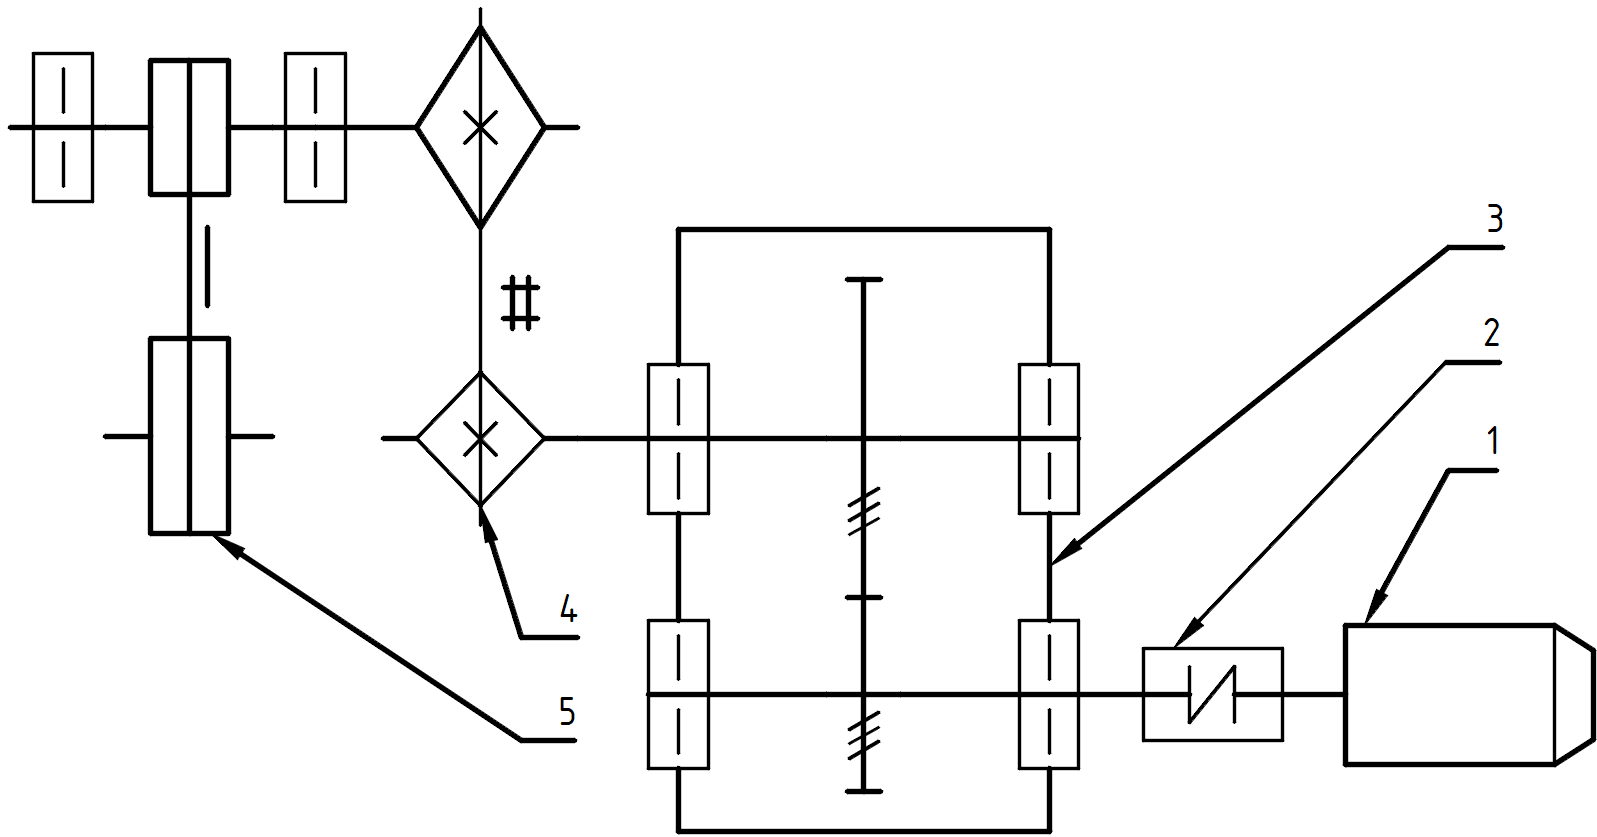
\includegraphics[width=150mm]{system.png}
%			\caption{Mechanical transmission system of a belt conveyor}
%			\label{system diagram}
%		\end{figure}
%	
%		\begin{figure}[ht]
%			\centering
%			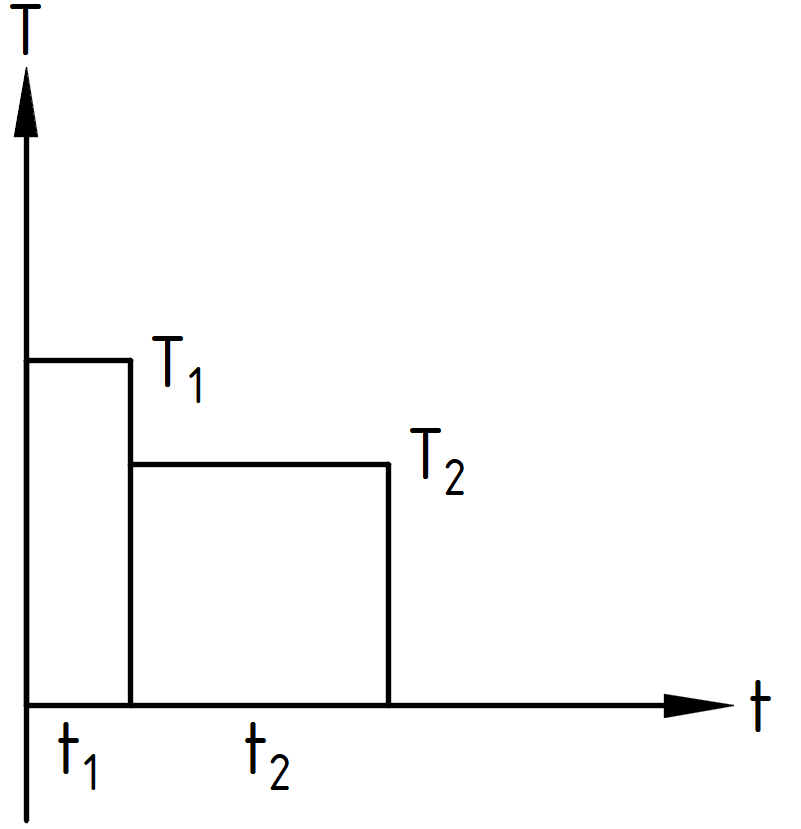
\includegraphics[width=70mm]{load.png}
%			\caption{Input load diagram}
%			\label{load diagram}
%		\end{figure}
%		Given the mechanical transmission system in figure \ref{system diagram}, determine the specifications for each machine element.
%		\begin{enumerate}
%			\item Electric motor
%			\item Elastic coupling
%			\item Gearbox
%			\item Chain drive
%			\item Belt conveyor
%		\end{enumerate}
%	
%		\paragraph{Design parameters} The chosen parameters are given in column 8:
%		\begin{itemize}
%			\item $ F_t = 4500 \unit{(N)} $
%			\item $ v_{bc} = 3.05 \unit{(m/s)} $
%			\item $ D_{bc} = 500 \unit{(mm)} $
%			\item $ L = 4 \unit{(years)} $
%			\item $ T_1 = T \unit{(N\cdot mm)}$, $ t_1 = 12 \unit{(s)} $
%			\item $ T_2 = 0.7T \unit{(N\cdot mm)}$, $ t_2 = 60 \unit{(s)} $
%			\item $ \delta_u \leq \pm 5\% $
%		\end{itemize}
%		The machine works in one direction for 300 days, 2 shifts per day, 8 hours each and the load is low. Also, for the rest of this report, we will consider shaft 1 is the one connected to the electric motor, while shaft 2 is the connection between the chain drive and gearbox.
	\chapter{Characteristics of a sensor}
When designing a mechatronic system, sensor is crucial for data acquisition and generating an adequate response. However, if a engineer only relies on the best available sensor, the product price will be higher than necessary, resulting in customers lost to competitive manufacturers. Therefore, this chapter is dedicated to accommodate selecting the right sensor for one's application with common characteristics available on datasheets.

\section{Mobile Communication Devices}
\begin{figure}[ht]
	\centering
	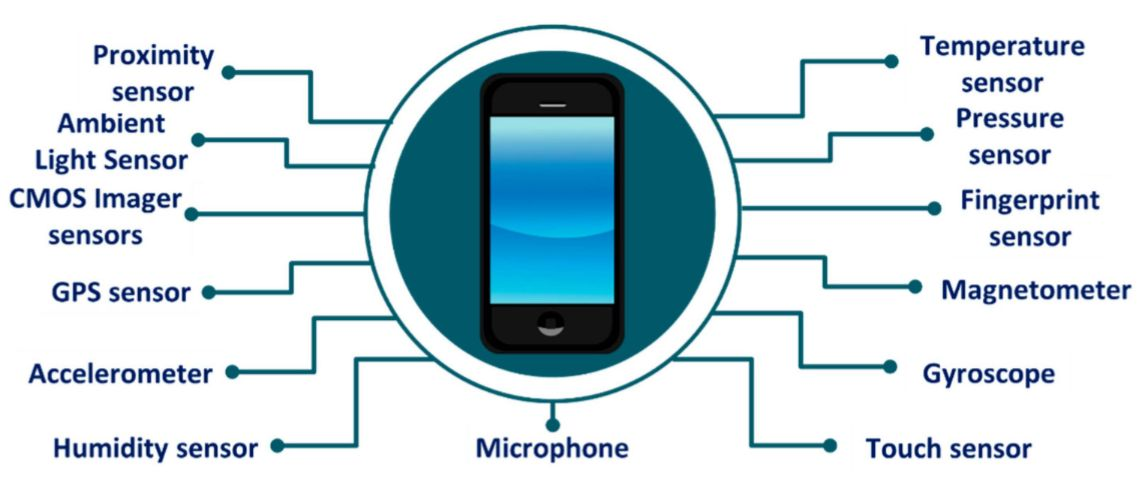
\includegraphics{mcd}
	\caption{Built-in sensors in a typical present-day smartphone}
\end{figure}
Mobile Communication Devices (MCD) sensors are designed for portability and full integration with other components inside a hand-held device. It is a self-containing sensing module that detects, conditions, digitizes, processes, outputs and communicates information while being small, light, accurate, stable, fast-response, etc. A generic purpose device (e.g. smartphones, tablets, smartwatches) contains dozens of them for different applications and is categorized in 4 areas:
\begin{enumerate}
	\item \textbf{Industrial} for detecting noncontact tempertaure, thermal imaging, humidity, air flow ionizing radiation, smell, diaelectric constant of objects, maerial composition, range (distance), air pressure, produce freshness, etc.
	\item \textbf{Medical} for the inner (core) and skin body temperatures, thermal imaging, arterial blood pressure, EKG, blood factors (glucose, cholesterol, hemoglobin oxygen saturation), deep body imaging, smell (e-nose), behavior modification, etc.
	\item \textbf{Military} for night vision, detecting poisonous gases, proximity, ionizing radiation, explosives, chemical and biological agents, etc.
	\item \textbf{Consumer} for the body core temperature, heart rate, radon gas, pregnancy detection, breathalizer for alcohol and hydrogen sulfide, food composition, behavior modification, proximity, V level, electromagnetic pollution, surface temperature, etc.
\end{enumerate}

\section{Full-Scale Input/Output}
A \textit{span} or an \textit{input full scale} (FS) is a dynamic range of stimuli convertible by a sensor. In a datasheet, it is regarded as the highest possible input value without causing unacceptably large error. For sensors with broad response characteristics, the span is often expressed in decibels, which is a logarithmic measure of ratios of either power or force (voltage).

A \textit{full-scale output} (FSO) for an analog output is the difference between electrical output signals at 2 ends of the input signals. For digital output, it is the maximum digital count the A/D converter can resolve for maximum FS.

\section{Accuracy}
It is defined as \textit{maximum}, or \textit{typical}, or \textit{average} error of the sensor alone. The rating of accuracy is represented in 4 common forms, depending on the application:
\begin{enumerate}
	\item \textit{Directly in terms of measured value of a stimulus}, which is used when error is independent on the input signal magnitude.
	\item \textit{In percentage of FS}, which is useful for a sensor with a linear transfer function and can be thought as an alternative of the approach above. For nonlinear transfer function, the representation may be misleading.
	\item \textit{In percentage of the measured signal}, which is useful for a nonlinear transfer function, even with very dynamic inputs. However, the error typically does not proportionally scale with the input magnitude.
	\item \textit{In terms of the output signal}, which is useful for sensors with a digital output format.
\end{enumerate}
In reality, a datasheet mixes 2 or more forms and take whichever value is the largest. In this way, the error can be evaluated more accurately.

\section{Possible types of error}
In a datasheet, tolerance and error limit are paramount for any measuring equipment, which the manufacture always dedicates a section for. Distinguishing the types of error is helpful to determine the suitable sensor for designing a mechatronic system. Generally, there are 6 types of error:
\paragraph{Calibration error}
Calibration error occurs while adjusting a sensor. In dynamic system and control, it is categorized as \textit{disturbance}, which is quantitative data and contributes the systematic error. Another source of errors regarding calibration is a reference sensor. This type of sensor is considered as national standard, which all manufactured sensors rely on. Therefore, for absolute accuracy, the error from "standardized sensors" is considered.
\paragraph{Hysteresis error}
Hysteresis error is the maximum deviation between output values given the same input signal. For example, if the sensitivity of the sensor is $ 10\unit{mV/mm} $, the hysteresis error in terms of displacement units is $ 2\unit{mm} $. Possible causes of this faulty result are geometry of design, friction or deformation of material.
\paragraph{Nonlinearity error}
If the error is assumed to , nonlinearity error will be specified to compensate for any faulty assumptions. It is the maximum deviation of a real transfer function from the approximation straight line. After several calibration runs, the worst linearity result is stated. This type of error is crucial if the output signal requires best accuracy in a small range (e.g. medical thermometer measures body temperature between $ 36-38^\circ\text{C} $). Oftentimes, manufacturers are inclined to publish the smallest possible nonlinearity error without specifying what approximation method is used.
\begin{figure}
	\centering
	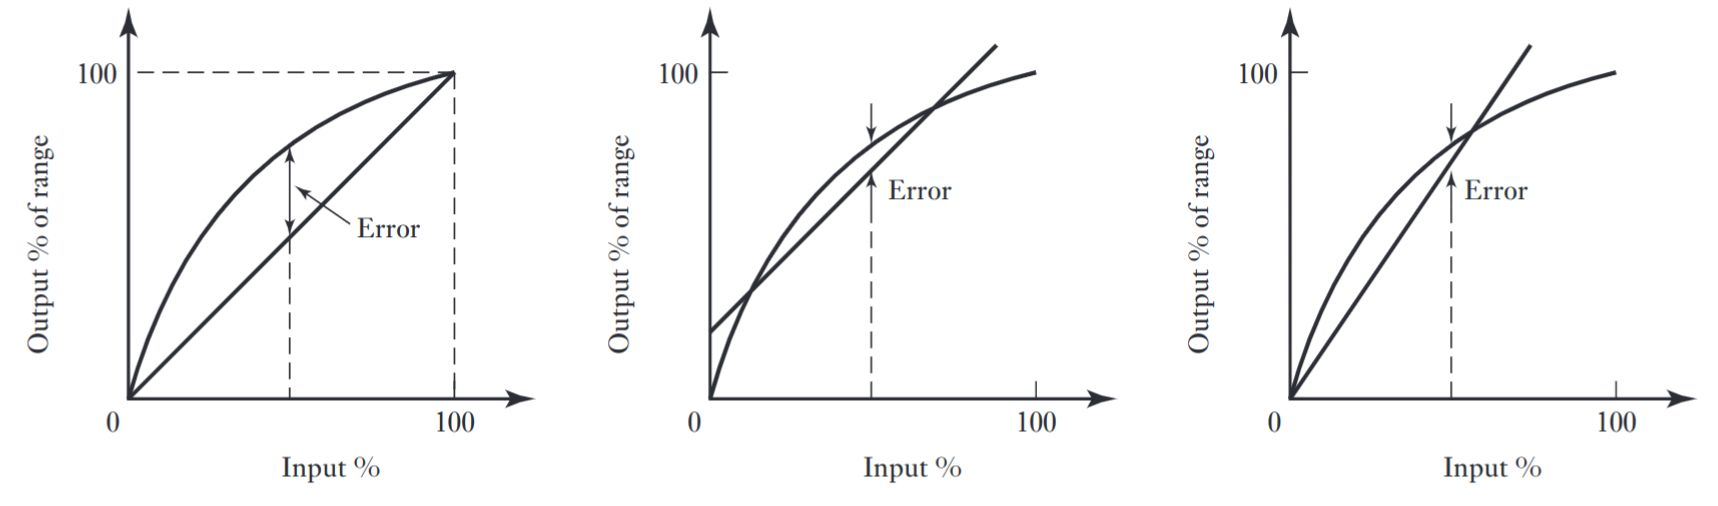
\includegraphics[width=\linewidth]{hysteresis}
	\caption{Non-linearity error using (from left to right): end-range values; best straight line for all values; best straight line through the zero point \cite{bolton2015mechatronics}}
\end{figure}
\paragraph{Saturation error}
Saturation error occurs when the input signal exceeds the operating limit of a sensor.
\paragraph{Repeatability error}
Repeatability error causes a sensor to output different values under identical conditions. Possible noises for the error are thermal conductivity, charge, deformation, etc.
\paragraph{Dead band error}
Dead band error is the insensitivity of a sensor in a specific range of the input signals, which generates output signals between a certain value (often zero).
\section{Resolution}
Digital input-output signals are not continuous as shown in the figures in a datasheet but rather distinguish data points. The distance between 2 consecutive data points is defined as resolution. Depending on manufacturers, the step size may be specified as typical, average, or worst.
\section{Special output characteristics}
Depending on sensor types, specifying input properties might be necessary. For instance, in case of flow sensors, thermal transport sensors require identifying temperature bandwidth to give the accurate response.
\paragraph{Impedance}
When working with an electronic sensor, the output impedance of the sensor $ Z_{out} $ and the input impedance of the connecting system $ Z_{in} $ should be acknowledge. A current generating sensor should have high $ Z_{out} $ and low $ Z_{in} $. This is the opposite for voltage generating sensor.
\paragraph{Format}
For mechatronic systems, programming a microcontroller or microprocessor needs the output format of the sensor. The output electrical characteristics may include voltage, current, charge, frequency, amplitude, phase, polarity, shape of a signal, time delay and digital code. These responses can be displayed in formats such as binary, text (ASCII), or digital output, etc. with various forms of communication (e.g. serial link, PWM, $ I^2C $).
\paragraph{Excitation}
Analogues to a match catching fire with a spark, excitation signal could be included in a datasheet. An exapmle of an excitation signal is electric current passing through a thermistor to measure its temperature-dependent resistance.
\paragraph{Dynamic characteristics}
Besides from steady input signals, dynamic and time-varying stimuli are also considered. The sensor responses slowly to this input type, which generates dynamic error. At best, the error is a delay. At worst, it causes undesirable oscillations. In such cases, Dynamic Systems and Control course is provided to discuss extensively about this topic.
\section{Environmental factors}
Generally, all possible environmental factors that may affect the sensor performance are specified by manufacturers. In a datasheet, it is typical to include information about the following factors:
\begin{enumerate}
	\item \textit{Storage condition}, which specifies the highest and lowest storage temperature. It also has maximum relative humidities at these temperatures and may be mentioned as "noncondensing". Along with operating temperature range, this information is \textit{one of the most common environmental factors} available in any datasheet. 
	\item \textit{Short-term stability} is manifested as changes in the sensor's performance within minutes, hours, or days, which essentially is another way to express bidirectional repeatability.
	\item \textit{Long-term stability} is the irreversible change in the material's electrical, mechanical, chemical or thermal properties. Similar to heat treated materials, a sensor can improve its stability by \textit{pre-aging}. For instance, a sensor may be periodically swung from freezing to hot temperatures before being calibrated and installed into a product.
	\item \textit{Environmental conditions during normal operation} affects the transfer function of a sensor. An example is a strain gauge whose sensitivity increases with temperature. Even if the manufacture does not specify these conditions in the datasheet, it is the responsibility of an engineer to simulate and prototype the end-product corresponding to the environment.
\end{enumerate}
\section{Reliability}
In statistical terms, reliability is the probability that the device will function without failure over a specified time or a number of uses. Reliability specifies a failure  is a temporary or permanent malfunction of a device. Although this is an important property of a sensor, the information is not readily available in most datasheet due to the absence of measuring standards of reliability. Therefore, an engineer should be ready to do the test by any means. Some example testing procedures are MTBF, extreme testing, accelerated life testing, HALT testing, FOAT testing, etc.
\section{Application characteristics}
This information includes geometry and other simple physical specifications such as design, weight, power consumption and overall dimensions. Although price heavily influences a sensor's performance, any amount of cost is justified if reliability and accuracy are of a paramount importance.
\section{Uncertainty}
While error is what we unknowably get when we measure, uncertainty is what we think how large that error might be. No matter how well a sensor is made, there always exists obscure factors. Even if they are recognized, it is impossible to measure exactly (e.g. human factor). Attempts have been made to quantitatively identify them: evaluation through statistical methods, preceding measurement data, personal experience, manufacturer's specifications, uncertainty data referenced from handbooks and manuals, etc.

	\chapter{Chapter 2 - appendix}
\section{section 1}
\section{section 2}

	\chapter{Gearbox Design (Helix gears)}
\section{Nomenclature}
	\begin{tabular}[t]{lp{6.5cm}}
		$ [\sigma_H] $ & permissible contact stress, $ \unit{MPa} $\\
		$ [\sigma_H]_{max} $ & permissible contact stress due to overload, $ \unit{MPa} $\\
		$ [\sigma_F] $ & permissible bending stress, $ \unit{MPa} $\\
		$ [\sigma_F]_{max} $ & permissible bending stress due to overload, $ \unit{MPa} $\\
		$ \text{AG} $ & accuracy grade of gear\\
		$ a $ & center distance, $ \unit{mm} $\\
		$ b $ & face width, $ \unit{mm} $\\
		$ c $ & gear meshing rate\\
		$ d $ & pitch circle, $ \unit{mm} $\\
		$ d_a $ & addendum diameter, $ \unit{mm} $\\
		$ d_b $ & base diameter, $ \unit{mm} $\\
		$ d_f $ & deddendum diameter, $ \unit{mm} $\\
		$ F_a $ & axial force, $ \unit{N} $\\
	\end{tabular}
	\begin{tabular}[t]{lp{6.5cm}}
		$ F_r $ & radial force, $ \unit{N} $\\
		$ F_t $ & tangential force, $ \unit{N} $\\
		$ H $ & surface roughness, HB\\
		$ K_d $ & coefficient of gear material\\	
		$ K_F $ & load factor from bending stress\\
		$ K_{FC} $ & load placement factor\\
		$ K_{FL} $ & aging factor due to bending stress\\
		$ K_{Fv} $ & factor of dynamic load from bending stress at meshing area\\
		$ K_{F\alpha} $ & factor of load distribution from bending stress on gear teeth\\
		$ K_{F\beta} $ & factor of load distribution from bending stress on top land\\
		$ K_H $ & load factor of contact stress\\
	\end{tabular}\newpage
\begin{tabular}[t]{lp{6.5cm}}
	$ K_{HL} $ & aging factor due to contact stress\\
	$ K_{Hv} $ & factor of dynamic load from contact stress at meshing area\\
	$ K_{H\alpha} $ & factor of load distribution from contact stress on gear teeth\\
	$ K_{H\beta} $ & factor of load distribution from contact stress on top land\\
	$ k_x $ & a coefficient\\
	$ k_y $ & a coefficient\\
	$ m $ & traverse module, $ \unit{mm} $\\
	$ m_F $ & root of fatigue curve in bending stress test\\
	$ m_H $ & root of fatigue curve in contact stress test\\
	$ m_n $ & normal module, $ \unit{mm} $\\
	$ N_{FE} $ & working cycle of equivalent tensile stress corresponding to $ [\sigma_F] $\\
	$ N_{FO} $ & working cycle of bearing stress corresponding to $ [\sigma_F] $\\
	$ N_{HE} $ & working cycle of equivalent tensile stress corresponding to $ [\sigma_H] $\\
	$ N_{HO} $ & working cycle of bearing stress corresponding to $ [\sigma_H] $\\
	$ S $ & specific length, $ \unit{mm} $\\
	$ S_F $ & safety factor of bending stress\\
		$ S_H $ & safety factor of contact stress\\
\end{tabular}
\begin{tabular}[t]{lp{6.5cm}}
	

	$ T $ & input torque, $ \unit{N\cdot mm} $\\
	$ v $ & rotational velocity, $ \unit{m/s} $\\
	$ x $ & gear correction factor\\
	$ Y_F $ & tooth shape factor\\
	$ Y_\beta $ & helix angle factor\\
	$ Y_\varepsilon $ & contact ratio factor\\
	$ y $ & center displacement factor\\
	$ z_H $ & contact surface's shape factor\\
	$ z_M $ & material's mechanical properties factor \\
	$ z_{min} $ & minimum number of teeth corresponding to $ \beta $\\
	$ z_v $ & virtual number of teeth\\
	$ z_\varepsilon $ & meshing condition factor\\
	$ \alpha $ & normal pressure angle, following Vietnam standard (TCVN 1065-71), i.e. $ \alpha = 20^\circ $\\
	$ \alpha_t $ & traverse pressure angle, $ ^\circ $\\
	$ \varepsilon_\alpha $ & traverse contact ratio\\
	$ \varepsilon_\beta $ & face contact ratio\\
	$ \beta $ & helix angle, $ ^\circ $\\
	$ \beta_b $ & base circle helix angle, $ ^\circ $\\
	$ \psi_{ba} $ & width to shaft distance ratio\\
	$ \psi_{bd} $ & face width factor \\
	$ \sigma_b $ & ultimate strength, $ \unit{MPa} $\\
	$ \sigma_{ch} $ & yield limit, $ \unit{MPa} $\\
	
\end{tabular}\newpage
\begin{tabular}[t]{lp{6.5cm}}
	$ \sigma_{Flim}^o $ & permissible bending stress corresponding to working cycle, $ \unit{MPa} $\\
	$ \sigma_{Hlim}^o $ & permissible contact stress corresponding to working cycle, $ \unit{MPa} $\\
\end{tabular}
\begin{tabular}[t]{lp{6.5cm}}
	
	$ _1 $ & subscript for pinion\\
	$ _2 $ & subscript for driven gear\\
	$ _w $ & subscript for variable value after correction\\
\end{tabular}

\section{Choose material}
From table (6.1) , the material of choice for both gears is steel 40X with $ S\leq100\unit{(mm)} $, $ \text{HB} 250 $, $ \sigma_b = 850\unit{(MPa)} $, $ \sigma_{ch} = 550 \unit{(MPa)}$.\\
Table (6.2)  also gives $ \sigma_{Hlim}^o = 2\text{HB} + 70$, $ S_H = 1.1 $, $ \sigma_{Flim}^o = 1.8\text{HB} $, $ S_F = 1.75 $\\
Therefore, they have the same properties except for their surface roughness $ H $. The reasoning is given on p.91, where $ H_2 = H_1 - 10 \div 15$ \\
For the pinion, $ H_1=\text{HB}250 \Rightarrow \sigma_{Hlim1}^o = 570\unit{(MPa)}$, $ \sigma_{Flim1}^o = 450\unit{(MPa)}$\\
For the driven gear, $ H_2=\text{HB}240 \Rightarrow \sigma_{Hlim2}^o = 550\unit{(MPa)}$, $ \sigma_{Flim2}^o = 432\unit{(MPa)}$

\section{Calculate $ [\sigma_H] $ and $ [\sigma_F] $}

\subsection{Working cycle of bearing stress}
Using equation (6.5) :\\
$ N_{HO1} = 30H_1^{2.4} = 17.07\times10^6\unit{(cycles)}$\\
$ N_{HO2} = 30H_2^{2.4} = 15.4749\times10^6\unit{(cycles)}$

\subsection{Working cycle of equivalent tensile stress}
Since $ H_1,H_2\leq\text{HB}350 $, $ m_H=6 $, $ m_F=6 $.\\
Both gears meshed indefinitely, thus $ c=1 $.\\
From working condition, we calculate:\\
$ L_h = 8\unit{\left( \dfrac{hours}{shift}\right)}\times2\unit{\left( \dfrac{shifts}{day}\right) }\times300\unit{\left( \dfrac{days}{year}\right)}\times4\unit{(years)}=19200\unit{(hours)}$\\
Applying equation (6.7)  and $ T_1 $, $ T_2 $, $ t_1 $, $ t_2 $ in the initial parameters:\\
$ N_{HE1} = 60n_{sh1}cL_h\left[ \left( \dfrac{T_1}{T}\right)^3\dfrac{t_1}{t_1+t_2} + \left( \dfrac{T_2}{T}\right)^3\dfrac{t_2}{t_1+t_2}\right] \approx 1.53\times10^9\unit{(cycles)}$\\
$ N_{HE2} = 60n_{sh2}cL_h\left[ \left( \dfrac{T_1}{T}\right)^3\dfrac{t_1}{t_1+t_2} + \left( \dfrac{T_2}{T}\right)^3\dfrac{t_2}{t_1+t_2}\right] \approx 0.31\times10^9\unit{(cycles)}$\\
$ N_{FE1} = 60n_{sh1}cL_h\left[ \left( \dfrac{T_1}{T}\right)^{m_F}\dfrac{t_1}{t_1+t_2} + \left( \dfrac{T_2}{T}\right)^{m_F}\dfrac{t_2}{t_1+t_2}\right] \approx 0.89\times10^9\unit{(cycles)}$\\
$ N_{FE2} = 60n_{sh2}cL_h\left[ \left( \dfrac{T_1}{T}\right)^{m_F}\dfrac{t_1}{t_1+t_2} + \left( \dfrac{T_2}{T}\right)^{m_F}\dfrac{t_2}{t_1+t_2}\right] \approx 0.18\times10^9\unit{(cycles)}$

\subsection{Aging factor}
For steel, $ N_{FO1} = N_{FO2} = 4\times10^6\unit{(MPa)}$. Applying equations (6.3) and (6.4)  yield (if $ K_{HL}, K_{FL} < 1 $, $ K_{HL} = 1$ and $ K_{FL} = 1$ according to the properties given on p.94):\\
$K_{HL1} = \sqrt[m_H]{N_{HO1}/N_{HE1}} \approx 0.47 < 1 \Rightarrow K_{HL1} = 1$\\
$ K_{HL2} = \sqrt[m_H]{N_{HO2}/N_{HE2}} \approx 0.61 < 1 \Rightarrow K_{HL2} = 1$\\
$ K_{FL1} = \sqrt[m_F]{N_{FO1}/N_{FE1}} \approx 0.41 < 1 \Rightarrow K_{FL1} = 1$\\
$ K_{FL2} = \sqrt[m_F]{N_{FO2}/N_{FE2}} \approx 0.53 < 1 \Rightarrow K_{FL2} = 1$

\subsection{Calculate $ [{\sigma}_H] $, $ [{\sigma}_{F1}] $, $ [{\sigma}_{F2}] $}
Since the motor works in one direction, $ K_{FC} = 1$. In ideal conditions, we assume $ Z_RZ_VK_{xH} = 1 $ and $ Y_RY_sK_{xF} = 1 $ according to p.92:\\
$ [{\sigma}_{H1}] = \sigma_{Hlim1}^oK_{HL1}/S_{H1} \approx 518.18 \unit{(MPa)}$\\
$ [{\sigma}_{H2}] = \sigma_{Hlim2}^oK_{HL2}/S_{H2} \approx 500 \unit{(MPa)}$\\
$ [{\sigma}_{F1}] = \sigma_{Flim1}^oK_{FC1}K_{FL1}/S_{F1} \approx 257.14\unit{(MPa)}$\\
$ [{\sigma}_{F2}] = \sigma_{Flim2}^oK_{FC2}K_{FL2}/S_{F2} \approx 246.86 \unit{(MPa)}$\\
The mean permissible contact stress must be lower than 1.25 times of either $ [{\sigma}_{H1}] $ or $ [{\sigma}_{H2}] $, whichever is smaller:\\
$ [{\sigma}_H] = \dfrac{1}{2}\left( [{\sigma}_{H1}]+[{\sigma}_{H2}]\right)  \approx 509.09 \unit{(MPa)}\leq 1.25[{\sigma}_H]_{min} = 1.25[{\sigma}_{H2}]$\\
The permissible contact stress and bending stress due to overload are calculated as follows:\\
$ [{\sigma}_H]_{max} = 2.8\sigma_{ch} = 1540\unit{(MPa)} $\\
$ [{\sigma}_F]_{max} = 0.8\sigma_{ch} = 440\unit{(MPa)} $

\section{Transmission Design}

\subsection{Determine basic parameters}
Examine table (6.5)  gives $ K_a = 43 $\\
Assuming symmetrical design, table (6.6)  also gives $ \psi_{ba} = 0.5$\\
$ \Rightarrow \psi_{bd} = 0.53\psi_{ba}(u_{hg}+1) = 1.59$\\
From table (6.7) , using interpolation, we approximate $ K_{H\beta} \approx 1.108 $, $ K_{F\beta} \approx 1.2558 $\\
Since the gear system only consists of involute gears and it is also a speed reducer gearbox, we estimate $ a $ using equation (6.15a) gives:\\
$ a = K_a(u_{hg}+1)\sqrt[3]{\dfrac{T_{sh1}K_{H\beta}}{[{\sigma}_H]^2u_{hg}\psi_{ba}}} \approx 113.7 \unit{(mm)}$\\
According to SEV229-75 standard, we choose $ a_w = 125 \unit{mm}$

\subsection{Determine gear meshing parameters}

\paragraph{Find $ m $} Applying equation (6.17)  and choose $ m $ from table (6.8) :\\
$ m = (0.01\div0.02)a_w = 1.25\div2.5 \unit{(mm)} \Rightarrow m=1.5\unit{(mm)}$

\paragraph{Find $ z_1 $, $ z_2 $, $ b_w $} Let $ \beta = 14^\circ $. Combining equation (6.18) and (6.20), we come up with the formula to calculate $ z_1 $. From the result, $ z_1 $ is rounded up to the nearest odd number (preferably a prime number).\\
$ z_1 = \dfrac{2a_w\cos\beta}{m(u_{hg}+1)} \approx 26.95 \Rightarrow z_1 = 27$\\
$ z_2 = u_{hg}z_1 = 135 $\\
$ \Rightarrow b = \psi_{ba}a_w = 62.5\unit{(mm)}$ 

\paragraph{Correct $ \beta $} There are 2 approaches for correction involving the change of either $ \alpha $ or $ \beta $. Because altering $ \alpha $ leads to many other corrections ($ d_1 $, $ d_2 $ and $ a_w $), $ \beta $ will be used instead.\\
Since $ z_1 $ is rounded, we must find $ \beta $ to obtain the correct angle, ensuring that $ \beta \in (8^\circ, 20^\circ) $. Using equation (6.32):\\
$ \beta_w = \arccos\dfrac{m(z_1+z_2)}{2a_w} \approx 13.59^\circ$

\paragraph{Find $ x_1 $, $ x_2 $} To find $ x_1 $ and $ x_2 $, we will follow the calculation scheme provided in p.103. Since $ \beta_w \approx 13.59^\circ \in (12,17]$, $ z_{min} = 16$, which leads to $ z_1 $ satisfying condition $ z_1 \geq z_{min} + 2 > 10 $, according to table (6.9). Combined with $ u_{hg} = 5 \geq 3.5 $, we obtain $ x_1 = 0.3 $, $ x_2 = -0.3 $, disregarding the calculation of $ y $.

\subsection{Basic parameters}

\begin{tabular}[t]{p{8cm}}
	$ d_1 = d_{w1} = \dfrac{mz_1}{\cos\beta} \approx 41.67\unit{(mm)} $\\
	$ d_2 = d_{w2} = \dfrac{mz_2}{\cos\beta} \approx 208.33 \unit{(mm)} $\\
	$ d_{a1} = d_1 + 2(1+x_1)m \approx 45.57\unit{(mm)}$\\
	$ d_{a2} = d_2 + 2(1+x_2)m \approx 210.43\unit{(mm)}$\\
	$ d_{f1} = d_1 - (2.5-2x_1)m \approx 38.82\unit{(mm)}$\\
	$ d_{f2} = d_2 - (2.5-2x_2)m \approx 203.68\unit{(mm)}$\\
\end{tabular}
\begin{tabular}[t]{p{8cm}}
	$ d_{b1} = d_1\cos\alpha \approx 39.15\unit{(mm)}$\\
	$ d_{b2} = d_2\cos\alpha \approx 195.77 \unit{(mm)}$\\
	$ \alpha_t = \alpha_{tw} = \arctan\dfrac{\tan\alpha}{\cos\beta_w} \approx 20.53^\circ $\\
	$ v = \dfrac{\pi d_1n_{sh1}}{6\times10^4} \approx 6.39\unit{(m/s)}$
\end{tabular}

\subsection{Find $ [{\sigma}_{Hw}] $, $ [\sigma_{Fw1}] $ and $ [\sigma_{Fw2}] $}
In this section, we will try to approximate these parameters based on the factors $ Z_R$, $Z_V$, $K_{xH} $ and $ Y_R$, $Y_s$, $K_{xF} $ to substitute to equation (6.1) and (6.2):
\[
\begin{array}{l@{{} = {}}l}
[\sigma_{Hw}] & [{\sigma}_H]Z_RZ_VK_{xH}\\

[\sigma_{Fw}] & [{\sigma}_F]Y_RY_SK_{xF}\\
\end{array}
\]
Assuming smooth surface condition, $ Z_R = 1 $.\\
$ Z_V = 0.85v^{0.1} \approx 1.02$ with $ H\leq350 $.\\
In case of $ v>5\unit{(m/s)} $, $ K_{xH} = 1$.\\
The pair of gears are properly polished, which makes $ Y_R=1.1 $\\
$ Y_s = 1.08-0.0695\ln(m) \approx 1.05 $\\
Since $ d_{a1},d_{a2}\leq400\unit{(mm)} $, $ K_{xF}=1 $, which leads to:\\
$ [{\sigma}_{Hw}] = 520.93\unit{(MPa)}$\\
$ [{\sigma}_{Fw1}] = 297.51\unit{(MPa)}$\\
$ [{\sigma}_{Fw2}] = 285.61\unit{(MPa)}$

\subsection{Contact stress analysis}
From section 6.3.3. in the text, contact stress applied on a gear surface must satisfy the condition below:
\[
	\sigma_H = z_Mz_Hz_\varepsilon\sqrt{2T_{sh1}K_H\dfrac{u_{hg}+1}{bu_{hg}d_{w1}^2}} \leq [{\sigma}_{Hw}]
\]

\paragraph{Find $ z_M $}
$ z_M = 274 $, according to table (6.5) 
\paragraph{Find $ z_H $}
$ \beta_b = \arctan\left( \cos\alpha_t\tan\beta_w\right) \approx 12.76^\circ \Rightarrow z_H = \sqrt{2\dfrac{\cos\beta_{b}}{\sin(2\alpha_{tw})}} \approx 1.72$
\paragraph{Find $ z_\varepsilon $} Obtaining $ z_\varepsilon $ through calculations:\\
$ \varepsilon_\alpha = \dfrac{\sqrt{d_{a1}^2-d_{b1}^2}+\sqrt{d_{a2}^2-d_{b2}^2}-2a_w\sin\alpha_{tw}}{2\pi m\dfrac{\cos\alpha_t}{\cos\beta_w}} \approx 1.41$\\
$ \varepsilon_\beta = b\dfrac{\sin\beta_w}{m\pi} \approx 3.12>1 \Rightarrow z_\varepsilon = \varepsilon_\alpha^{-0.5} \approx 0.86 $
\paragraph{Find $ K_H $} We find $ K_H $ using equation $ K_H = K_{H\beta}K_{H\alpha}K_{Hv} $\\
From table (6.13), $ v\leq 10 \unit{(m/s)}\Rightarrow \text{AG} = 8 $ \\
From table (P2.3), using interpolation, we approximate:\\ $ K_{Hv} \approx1.07$, $ K_{Fv} \approx1.18$\\
From table (6.14), using interpolation, we approximate:\\ $ K_{H\alpha} \approx1.1$, $ K_{F\alpha} \approx1.29 $ \\	
$ \Rightarrow K_H \approx 1.3 $
\paragraph{Find $ \sigma_H $} After calculating $ z_M $, $ z_H $, $ z_\varepsilon $, $ K_H $, we get the following result:
	\[\sigma_H \approx 477.51 \unit{(MPa)}\leq [{\sigma}_{Hw}] \approx 509.09 \unit{(MPa)}\] 

\subsection{Bending stress analysis}
For safety reasons, the following conditions must be met:
\[
\begin{array}{l@{{} \leq {}}l}
	\sigma_{F1} = 2\dfrac{T_{sh1}K_FY_\varepsilon Y_\beta Y_{F1}}{bd_{w1}m_n} & [\sigma_{Fw1}]\\ 
	\sigma_{F2} = \dfrac{\sigma_{F1}Y_{F2}}{Y_{F1}} & [\sigma_{Fw2}]
\end{array}
\]

\paragraph{Find $ Y_\varepsilon $} Knowing that $ \varepsilon_\alpha \approx 1.41 $, we can calculate $ Y_\varepsilon = \varepsilon_\alpha^{-1} \approx 0.71 $
\paragraph{Find $ Y_\beta $} $ Y_\beta = 1-\dfrac{\beta_w}{140}\approx0.9$
\paragraph{Find $ Y_F $} Using formula $ z_v = z\cos^{-3}(\beta_w) $ and table (6.18):\\
$ z_{v1} = z_1\cos^{-3}(\beta_w) \approx 29.4 \Rightarrow Y_{F1} \approx 3.54$\\
$ z_{v2} = z_2\cos^{-3}(\beta_w) \approx 147.01 \Rightarrow Y_{F2} \approx 3.63 $
\paragraph{Find $ K_F $}
Using $ K_{F\beta} $, $ K_{F\alpha} $, $ K_{Fv} $ calculated from the sections above, we derive:\\ $ K_F = K_{F\beta}K_{F\alpha}K_{Fv} \approx 1.91 $

\paragraph{Find $ \sigma_F $} Since $ m_n = m\cos\beta_w \approx 1.46$, substituting all the values, we find out that:
\begin{align*}
	\sigma_{F1} \approx 130.83 \unit{(MPa)} & \leq [\sigma_{Fw1}]\approx 297.51 \unit{(MPa)}\\
	\sigma_{F2} \approx 115.98 \unit{(MPa)} & \leq [\sigma_{Fw2}]\approx 285.61 \unit{(MPa)}
\end{align*}

\subsection{Force on shafts}
$ F_t = \dfrac{2T_{sh1}}{d_{w1}} \approx 2402.28 \unit{(N)}$\\
$ F_r = F_t\tan\alpha_{tw} \approx 899.55 \unit{(N)}$\\
$ F_a = F_t\tan\beta_w\approx 580.75 \unit{(N)}$\\
In summary, we have the following table:
\begin{table}[ht]
	\centering
	\begin{tabular}[t]{|
			>{\columncolor[HTML]{C0C0C0}}l |p{2.5cm}|p{2.5cm}|}
		\hline
		& \multicolumn{1}{c|}{\cellcolor[HTML]{C0C0C0}pinion} & \multicolumn{1}{c|}{\cellcolor[HTML]{C0C0C0}driving gear} \\ \hline
		$ H\unit{(HB)} $              & 250                      & 240    \\ \hline
		$ [\sigma_F]\unit{(MPa)} $    & 257.14                   & 246.86 \\ \hline
		$ [{\sigma}_H]\unit{(MPa)} $    & \multicolumn{2}{l|}{\hskip2cm 509.09}       \\ \hline
		$ [\sigma_H]_{max}\unit{(MPa)} $    & \multicolumn{2}{l|}{\hskip2cm 1540}       \\ \hline
		$ [\sigma_F]_{max}\unit{(MPa)} $    & \multicolumn{2}{l|}{\hskip2cm 440}       \\ \hline
		$ a_w\unit{(mm)} $            & \multicolumn{2}{l|}{\hskip2cm 100}           \\ \hline
		$ b\unit{(mm)} $            & \multicolumn{2}{l|}{\hskip2cm 50}           \\ \hline
		$ m\unit{(mm)} $              & \multicolumn{2}{l|}{\hskip2cm 1.5}    \\ \hline
		$ d_w\unit{(mm)} $              & 33.33                    & 166.67 \\ \hline
		$ d_a\unit{(mm)} $            & 37.23                    & 168.77 \\ \hline
		$ d_f\unit{(mm)} $            & 30.48                    & 162.02 \\ \hline
		$ d_b\unit{(mm)} $            & 31.32                     & 156.62 \\ \hline
		$ u_{hg} $              & \multicolumn{2}{l|}{\hskip2cm 5}    \\ \hline
		$ v\unit{(m/s)} $              & \multicolumn{2}{l|}{\hskip2cm 5}    \\ \hline
		$ x\unit{(mm)} $                       & 0.3                       & -0.3     \\ \hline
		$ z $                       & 21                       & 105     \\ \hline
		$ \alpha_{tw}\unit{(^\circ)} $ & \multicolumn{2}{l|}{\hskip2cm 20.65}        \\ \hline
		$ \beta_w\unit{(^\circ)} $ & \multicolumn{2}{l|}{\hskip2cm 19.09}        \\ \hline
	\end{tabular}
	\caption{Gearbox specifications}
\end{table}
	\chapter{Shaft Design}
\section{Nomenclature	}
\section{Choose material}
We choose material based on the following formula:
\[v_s=4.5\times10^{-5}n\sqrt[3]{T}\]
With $ n_{sh1} = 2930\unit{rpm} $, $ T_{sh1} \approx 37570.93\unit{N\cdot mm} \Rightarrow v_{s1} \approx 4.42 \unit{m/s}$\\
With $ n_{sh2} = 586\unit{rpm} $, $ T_{sh2} \approx 178537.08\unit{N\cdot mm} \Rightarrow v_{s2} \approx 1.48 \unit{m/s}$\\
Therefore, for shaft 1, we choose worm wheel material \foreignlanguage{russian}{бра жн} 10-4-4, which yields $ \sigma_{b1}=600\unit{MPa} $, $ \sigma_{ch1} = 200\unit{MPa} $ according to table 7.1. Using interpolation and table 7.2, the choice of shaft material is quenched and tempered 45 steel (specifications in table 6.1), which yields $ [\sigma_{H1}] \approx 191.3259 \unit{MPa}$.\\
For shaft 2, we choose worm wheel material \foreignlanguage{russian}{сч} 15-32, which yields $ \sigma_{b2}=150\unit{MPa} $, $ \sigma_{ch2} = 320\unit{MPa} $ according to table 7.1. Also using interpolation and table 7.2, the choice of shaft material is 20X steel (specifications in table 6.1), which yields $ [\sigma_{H2}] \approx 141.7534 \unit{MPa}$.

\section{Determine permissible stress}

\subsection{Find $ [\sigma_H] $}
Since $v_{s1} \approx 4.42 \unit{m/s} < 5\unit{m/s}$ and $v_{s2} \approx 1.48 \unit{m/s} < 2\unit{m/s}$, table 7.2 is used to find $ [\sigma_H] $. From the results above, we choose:\\
$ [\sigma_{H1}] \approx 191.3259 \unit{MPa}$\\
$ [\sigma_{H2}] \approx 141.7534 \unit{MPa}$

\subsection{Find $ [\sigma_F] $}
For shaft 1, we use the formula:
\[[\sigma_{F1}] = [\sigma_{FO1}]K_{FL1}\]
Since the steel is quenched, we can increase $ [\sigma_{FO1}] $ by $ 25\% $
$ [\sigma_{FO1}] = (0.25\sigma_{b1} + 0.08\sigma_{ch1})\times125\% = 207.5\unit{MPa} $\\
$ K_{FL1} = \sqrt[9]{10}$
	\chapter{Gear Design (shaft 2-3)}
%\section*{Nomenclature}
%\begin{tabular}[t]{p{0.1\linewidth}p{0.35\linewidth}}
%	$ [\sigma] $ & permissible stress, $ \unit{MPa} $\\
%	$ [\sigma]_{max} $ & permissible stress due to overloading, $ \unit{MPa} $\\
%	$ \text{AG} $ & accuracy grade of gear\\
%	$ a $ & center distance, $ \unit{mm} $\\
%	$ b $ & face width, $ \unit{mm} $\\
%	$ c $ & gear meshing rate\\
%	$ d $ & pitch circle, $ \unit{mm} $\\
%	$ d_a $ & addendum diameter, $ \unit{mm} $\\
%	$ d_b $ & base diameter, $ \unit{mm} $\\
%	$ d_f $ & deddendum diameter, $ \unit{mm} $\\
%	$ H $ & surface roughness, HB\\
%	$ K_d $ & coefficient of gear material\\	
%	$ K $ & overall load factor\\
%	$ K_{C} $ & load placement factor\\
%	$ K_{L} $ & aging factor\\
%	$ K_{v} $ & dynamic load factor at meshing area\\
%	$ K_{\alpha} $ & load distribution factor on gear teeth\\
%	$ K_{\beta} $ & load distribution factor on top land\\
%	$ K_{qt} $ & overloading factor\\
%	$ m $ & root of fatigue curve in stress test\\
%	$ m_t $ & traverse module, $ \unit{mm} $\\
%	
%%	$ F_a $ & axial force, $ \unit{N} $\\
%%	$ F_r $ & radial force, $ \unit{N} $\\
%%	$ F_t $ & tangential force, $ \unit{N} $\\
%\end{tabular}
%\begin{tabular}[t]{p{0.05\linewidth}p{0.4\linewidth}}
%	$ m_n $ & normal module, $ \unit{mm} $\\
%	$ N_{E} $ & working cycle of equivalent tensile stress\\
%	$ N_{O} $ & working cycle of bearing stress\\
%	$ S $ & safety factor\\	
%	$ v $ & rotational velocity, $ \unit{m/s} $\\
%	$ Y_F $ & tooth shape factor\\
%	$ Y_R $ & surface roughness factor\\
%	$ Y_s $ & stress concentration factor\\
%	$ Y_\beta $ & helix angle factor\\
%	$ Y_\varepsilon $ & contact ratio factor\\
%	$ Z_R $ & surface roughness factor of the working's area\\
%	$ Z_v $ & speed factor\\
%	$ z_H $ & contact surface's shape factor\\
%	$ z_M $ & material's mechanical properties factor\\
%	$ z_v $ & virtual number of teeth\\
%	$ z_\varepsilon $ & meshing condition factor\\
%	$ \alpha $ & normal pressure angle. In TCVN 1065-71, $ \alpha = 20^\circ $\\
%	$ \alpha_t $ & traverse pressure angle, $ ^\circ $\\
%	$ \varepsilon_\alpha $ & traverse contact ratio\\
%	$ \varepsilon_\beta $ & face contact ratio\\
%	$ \beta $ & helix angle, $ ^\circ $\\
%\end{tabular}\newpage
%\noindent\begin{tabular}[t]{p{0.05\linewidth}p{0.4\linewidth}}
%	$ \beta_b $ & base circle helix angle, $ ^\circ $\\
%	$ \psi_{ba} $ & width to shaft distance ratio\\
%	$ \psi_{bd} $ & face width factor \\
%	$ \sigma_b $ & ultimate strength, $ \unit{MPa} $\\
%	$ \sigma_{ch} $ & yield limit, $ \unit{MPa} $\\
%	$ \sigma_{lim}^o $ & permissible stress corresponding to working cycle, $ \unit{MPa} $\\	
%\end{tabular}
%\begin{tabular}[t]{p{0.05\linewidth}p{0.4\linewidth}}
%	$ \sigma_{max} $ & stress due to overloading, $ \unit{MPa} $ \\
%	$ _{1} $ & subscript for the pinion \\
%	$ _{2} $ & subscript for the driven gear\\
%	$ _F $ & subscript relating to bending stress\\
%	$ _H $ & subscript relating to contact stress\\
%\end{tabular}

\section{Choose material}
For small scale machines, type I material, which is often quenched and has low hardness ($ \text{HB}\leq 350 $), is sufficient. Precise manufacture is possible albeit low permissible stresses. In this design problem, the gear drive uses quenched 45 steel, whose specification is displayed on Table 6.1 \cite{tk1}:
\begin{itemize}
	\item Brinell hardness $ \text{HB} 205 $
	\item ultimate strength $ \sigma_b = 600\unit{MPa} $
	\item yield limit $ \sigma_{ch} = 340 \unit{MPa}$
\end{itemize}

\section{Stress estimation}
From working condition, the service life in hours are
\[L_h = 8\unit{\left( \dfrac{hours}{shift}\right)}\times Ca  K_{ng} L= 8 \times 1\times 260\times 8 = 16640\unitp{hours}\]
where all parameters are given in the design problem.

Since many variables are different in both gears, it should be convenient to introduce 4 subscripts for the parameters. Unless otherwise stated,
\begin{itemize}
	\item subscript $ _1 $ denotes the pinion attached to shaft 2.
	\item subscript $ _2 $ denotes the driven gear attached to shaft 3.
	\item subscript $ _F $ denotes bending stress.
	\item subscript $ _H $ denotes contact stress.
\end{itemize}
\subsection{Estimate the permissible contact stress $ [\sigma_H] $ and bending stress $ [\sigma_F] $}
Preliminary estimation of the permissible stresses uses Equation 6.1a and 6.2a \cite{tk1}. The exact calculation is considered in the next section:
\[[\sigma_H]=\dfrac{\sigma_{Hlim}^o}{S_H}K_{HL}\]
\[[\sigma_F]=\dfrac{\sigma_{Flim}^o}{S_F}K_{FC}K_{FL}\]

%Preliminary estimation of these values assumes $ Z_RZ_vK_{xH} = 1 $ and $ Y_RY_sK_{xF} = 1 $. These factors will be accounted for in the next sections.

\paragraph{Find permissible stress corresponding to a working cycle $ \sigma_{lim}^o $}
The value depends on hardness. The pinion also should be harder than the driving gear $ \text{HB} 10 \div 15 $. For quenched 45 steel, the formulas below are used, Table 6.2 \cite{tk1}:
\[ \sigma_{Hlim}^o = 2\text{HB} + 70\]
\[ \sigma_{Flim}^o = 1.8\text{HB}\]

For the pinion with $ H_1=\text{HB}205$:
\[ \sigma_{Hlim1}^o = 2 \times 205 + 70 = 480 \unitp{MPa}\]
\[ \sigma_{Flim1}^o = 1.8\times 205 = 369 \unitp{MPa}\]

For the driven gear with $ H_2=H_1-15=205-15=\text{HB}190 $:
\[ \sigma_{Hlim2}^o = 2 \times 190 + 70 = 450 \unitp{MPa}\]
\[ \sigma_{Flim2}^o = 1.8\times 190 = 342 \unitp{MPa}\]

\paragraph{Find safety factor $ S $}
The safety factors $ S_H=1.1 $, $ S_F=1.75 $ depend on material type, Table 6.2 \cite{tk1}.

\paragraph{Find load placement factor $ K_{FC} $}
$ K_{FC} = 1$ for unidirectional operation (i.e. load placement is in one way).

\paragraph{Find aging factor $ K_L $}
The factor is determined by Equation 6.3 and 6.4 \cite{tk1} for contact stress and bending stress, respectively. If calculation yields a value smaller than 1, it is then rounded up to 1 instead, p.94 \cite{tk1}:\\
\[ K_{HL1} = \sqrt[m_H]{N_{HO1}/N_{HE1}} = \sqrt[6]{10600601.81/0.37 \times10^9} = 0.46 < 1 \Rightarrow K_{HL1} = 1\]
\[ K_{HL2} = \sqrt[m_H]{N_{HO2}/N_{HE2}} = \sqrt[6]{8833440.68/0.13 \times10^9} = 0.54 < 1 \Rightarrow K_{HL2} = 1\]
\[ K_{FL1} = \sqrt[m_F]{N_{FO1}/N_{FE1}} = \sqrt[6]{4000000/0.32 \times10^9} = 0.40 < 1 \Rightarrow K_{FL1} = 1\]
\[ K_{FL2} = \sqrt[m_F]{N_{FO2}/N_{FE2}} = \sqrt[6]{4000000/0.11 \times10^9} = 0.48 < 1 \Rightarrow K_{FL2} = 1\]
where
\begin{itemize}
	\item $ m $ is the root of fatigue curve in the stress test of a material. Since $ H_1,H_2 \leq 350 $, $ m_H=6 $ and $ m_F=6 $.
	\item $ N_O $ is the working cycle of equivalent bearing stress. Using Equation 6.5 \cite{tk1}:\\
	\[ N_{HO1} = 30H_1^{2.4} = 30\times 205^{2.4} = 10600601.81\unitp{cycles}\]
	\[ N_{HO2} = 30H_2^{2.4} = 30\times 190^{2.4} = 8833440.68\unitp{cycles}\]
	where all parameters are given in previous sections.
	
	For bending stress, $ N_{FO1}= N_{FO2}= 4000000\unitp{MPa}$ since both gears use steel material.
	\item $ N_E $ is the working cycle of equivalent tensile stress. From Equation 6.7 and 6.8 \cite{tk1}:
	\begin{flalign*}
	N_{HE1} &= 60n_{sh2}cL_h\left[ \left( \dfrac{T_1}{T}\right)^3\dfrac{t_1}{t_1+t_2} + \left( \dfrac{T_2}{T}\right)^3\dfrac{t_2}{t_1+t_2}\right] \\
	&= 60 \times 514.42 \times 1 \times 16640 \left[ \left( \dfrac{T}{T}\right)^3\dfrac{15}{15+11} + \left( \dfrac{0.7T}{T}\right)^3\dfrac{11}{15+11}\right] \\
	&= 0.37 \times10^9\unitp{cycles}
	\end{flalign*}
	\begin{flalign*}
	N_{HE2} &= 60n_{sh3}cL_h\left[ \left( \dfrac{T_1}{T}\right)^3\dfrac{t_1}{t_1+t_2} + \left( \dfrac{T_2}{T}\right)^3\dfrac{t_2}{t_1+t_2}\right]\\
	&= 60 \times 181.88 \times 1 \times 16640 \left[ \left( \dfrac{T}{T}\right)^6\dfrac{15}{15+11} + \left( \dfrac{0.7T}{T}\right)^6\dfrac{11}{15+11}\right] \\
	&= 0.13 \times10^9\unitp{cycles}
	\end{flalign*}
	\begin{flalign*}
	N_{FE1} &= 60n_{sh2}cL_h\left[ \left( \dfrac{T_1}{T}\right)^{m_F}\dfrac{t_1}{t_1+t_2} + \left( \dfrac{T_2}{T}\right)^{m_F}\dfrac{t_2}{t_1+t_2}\right] \\
	&= 60 \times 514.42 \times 1 \times 16640 \left[ \left( \dfrac{T}{T}\right)^6\dfrac{15}{15+11} + \left( \dfrac{0.7T}{T}\right)^6\dfrac{11}{15+11}\right]\\
	&= 0.32 \times10^9\unitp{cycles}
	\end{flalign*}
	\begin{flalign*} 
	N_{FE2} &= 60n_{sh3}cL_h\left[ \left( \dfrac{T_1}{T}\right)^{m_F}\dfrac{t_1}{t_1+t_2} + \left( \dfrac{T_2}{T}\right)^{m_F}\dfrac{t_2}{t_1+t_2}\right]\\
	&= 60 \times 181.88 \times 1 \times 16640 \left[ \left( \dfrac{T}{T}\right)^6\dfrac{15}{15+11} + \left( \dfrac{0.7T}{T}\right)^6\dfrac{11}{15+11}\right] \\
	&= 0.11 \times10^9\unitp{cycles}
	\end{flalign*}
	where\begin{itemize}
		\item $ c=1 $ is the gear meshing rate. The value $ 1 $ indicates the gears are meshed indefinitely.
		\item $ T_1,T_2,t_1,t_2 $ are given in the design problem.
		\item $ n_{sh2}, n_{sh3} $ are given in Chapter 1.
		\item $ L_h, m_F $ are given in previous sections.
	\end{itemize}
\end{itemize}

\paragraph{Calculate preliminary values of $ [\sigma_H] $, $ [\sigma_{F1}] $, $ [\sigma_{F2}] $} Replacing all the values gives:\\
\[ [\sigma_{H1}] = \sigma_{Hlim1}^oK_{HL1}/S_H = 480\times 1/1.1 = 436.36 \unitp{MPa}\]
\[ [\sigma_{H2}] = \sigma_{Hlim2}^oK_{HL2}/S_H = 450\times 1/1.1 = 409.09 \unitp{MPa}\]
\[ [\sigma_{F1}] = \sigma_{Flim1}^oK_{FC}K_{FL1}/S_F = 369\times 1\times 1/1.75  = 210.86\unitp{MPa}\]
\[ [\sigma_{F2}] = \sigma_{Flim2}^oK_{FC}K_{FL2}/S_F = 342\times 1\times 1/1.75  = 195.43 \unitp{MPa}\]

The permissible contact stress of the gear drive $ [\sigma_H] $ must be lower than 1.25 times of either $ [\sigma_{H1}] $ or $ [\sigma_{H2}] $, whichever is smaller. In this case, it is $ 1.25[\sigma_{H2}]$:
\begin{multline*}
[\sigma_H] =\dfrac{[\sigma_{H1}]+[\sigma_{H2}]}{2}= \dfrac{436.36+409.09}{2} = 422.73 \unitp{MPa}\\
\leq 1.25[\sigma_{H2}] = 1.25\times 409.09= 511.36\unitp{MPa}
\end{multline*}

\subsection{Find permissible contact stress $ [\sigma_H]_{max} $ and bending stress $ [\sigma_F]_{max} $ due to overload}
Preventing overload failure is necessary. For quenched material, the permissible overload contact stress $ [\sigma_H]_{max} $ is
\[ [\sigma_H]_{max} = 2.8\times \sigma_b = 2.8\times 600 = 952.00\unitp{MPa} \]

For material with hardness smaller than $ \text{HB}350 $, the permissible overload bending stress $ [\sigma_F]_{max} $ is
\[ [\sigma_F]_{max} = 0.8\sigma_{ch} = 0.8\times 340 = 272.00\unitp{MPa} \]

\section{Determine basic specifications of the transmission system}
Undercutting process is omitted due to complexity and maintenance. That is, it is not factored in any variables of the gear drive.
\subsection{Determine basic parameters}
\subsubsection{Find center distance $ a $}
For involute gears, the center distance $ a $ is estimated using Equation 6.15a \cite{tk1} and rounded up to a multiple of 5 (small production type, p.99 \cite{tk1}):
\begin{multline*}
a= K_a(u+1)\sqrt[3]{\dfrac{TK_{H\beta}}{[\sigma_H]^2u\psi_{ba}}}	=  43\times(2.83+1)\times\sqrt[3]{\dfrac{126093.30\times 1.08}{422.73^2\times 2.83\times 0.39}}\\
= 145.47 \unitp{mm} \Rightarrow a= 160 \unit{mm}
\end{multline*}
where
\begin{itemize}
	\item $ K_a=43 $ is the material factor, Table 6.5 \cite{tk1}. The helical gear drive made of steel (both gears) corresponds to the value in the table.
	\item $ u =u_1 = 2.83$ is the speed ratio of the gear drive, which is given in Chapter 1.
	\item $ T=T_{sh2}= 126093.30\unit{N\cdot mm}$ is the torque exerted on the pinion, which is transmitted from the motor to shaft 1.
	\item $ K_{H\beta} = 1.08 $ is the load distribution factor on gear teeth, Table 6.7 \cite{tk1}. In the table, the gear placement in the speed reducer is similar to diagram 4
	\item $ \psi_{ba} = 0.39 $ is the width to shaft distance ratio, Table 6.6 \cite{tk1}. The pinion is asymmetrical about the bearings and both gears surface have hardness smaller than $ \text{HB}350 $. The value is obtained after extensive calculation and changing parameters, which includes hardness, center distance and traverse module. In addition, the remaining gear drive contributes to $ \psi_{ba} $, eventually reducing the center distance further, saving material cost.
	\item $ [\sigma_H] $ is given in previous section.
\end{itemize}

\subsubsection{Find face width ratio $ \psi_{bd} $}
$ \psi_{bd} $ is the face width factor. Using Equation 6.16 \cite{tk1}:
\[ \psi_{bd} = 0.53\psi_{ba}(u+1) = 0.53\times 0.39\times(2.83+1) = 0.80 \]
where all parameters are identified. The calculated value satisfies even with the minimum permissible factor  $ \psi_{bdmax} = 1 $, Table 6.6 \cite{tk1}.
%Figure \ref{fig:problem} shows both pairs are helical, which  gives $ K_a = 43 $, Table 6.5 \cite{tk1}. Also, the pinion is , resulting in $ \psi_{ba} $, . Then, $ \psi_{bd} $ is calculated using Equation 6.16 \cite{tk1}:\\
%, which is smaller than the permissible ratio $ \psi_{bdmax}=1.2 $, Table 6.6 \cite{tk1}.
%
%The gear placement in the speed reducer is similar to diagram 4 of Table 6.7 \cite{tk1}. $ K_{H\beta} = 1.08 $, $ K_{F\beta} = 1.1 $
\subsubsection{Find traverse module $ m_t $}
Using Equation 6.17 and Table 6.8 \cite{tk1}, the traverse module $ m $ is
\[ m_t = (0.01\div0.02)a = (0.01\div0.02)\times 160 =  1.6 \div 3.2 \unitp{mm} \Rightarrow m_t=3.00\unit{mm}\]

The choice is based on calculation to satisfy strength condition, as mentioned in choosing $ \psi_{ba} $.
\subsubsection{Find number of teeth $ z $}
Through calculation, helix angle $ \beta = 20^\circ $ should be preferred (permissible value is $ 8 \div 20^\circ $). Using Equation 6.31 and 6.20 \cite{tk1}, the pinion's number of teeth $ z_1 $ is
\[ z_1 = \dfrac{2a\cos\beta}{m_t(u+1)}= \dfrac{2\times 160\cos 20^\circ}{3.00\times(2.83+1)} = 26.18 \Rightarrow z_1 = 27\]
\[ z_2 = uz_1 = 2.83\times 27 = 76.37 \Rightarrow z_2 = 77\]
where all parameters are given in previous sections. The number of teeth selection follows the \textit{hunting tooth ratio} \cite{Ishibashi1981} as mentioned in Chapter 1. The ratio yields $ z_2/z_1=77/27=2.852 $, which is essentially not much different from the intended value $ u =2.83$. 

\subsubsection{Correct $ \beta $} The helix angles are corrected to compensate for rounding center distance and number of teeth, Equation 6.32 \cite{tk1}:
\[\beta = \arccos\dfrac{m_t(z_2+z_1)}{2a} = \arccos\dfrac{3.00\times(77+27)}{2\times 160} = 12.84 ^\circ\]

\subsection{Other parameters}
The values below are necessary for modeling the gear drive:\\
\[ b = \psi_{ba}a = 0.39\times 160= 62.40\unitp{mm}\]
\[ d_1 = {m_tz_1}/{\cos\beta} = {3.00\times 27}/{\cos9.07^\circ} = 83.08\unitp{mm}\]
\[ d_2 = {m_tz_2}/{\cos\beta} = {3.00\times 77}/{\cos9.07^\circ} = 236.92\unitp{mm}\]
\[ d_{a1} = d_1 + 2m_t = 83.08 + 2\times 3.00 = 89.08\unitp{mm}\]
\[ d_{a2} = d_2 + 2m_t = 236.92 + 2\times 3.00 = 242.92\unitp{mm}\]
\[ d_{b1} = d_1\cos\alpha = 83.08\times \cos 20^\circ = 78.07\unitp{mm}\]
\[ d_{b2} = d_2\cos\alpha = 236.92\times \cos 20^\circ = 222.63 \unitp{mm}\]
\[ d_{f1} = d_1 - 2.5m_t = 83.08 - 2.5\times 3.00 = 75.58\unitp{mm}\]
\[ d_{f2} = d_2 - 2.5m_t = 236.92 - 2.5\times 3.00 = 229.42\unitp{mm}\]
\[ \alpha_t = \arctan\left({\tan\alpha}/{\cos\beta}\right) = \arctan\left({\tan 20^\circ}/{\cos 12.84^\circ}\right) = 20.47^\circ\]
\[ v_1 = {\pi d_1n_{sh2}}/{60000} = {\pi \times 83.08 \times 514.42}/{60000} = 2.24\unitp{m/s}\]
where
\begin{itemize}
	\item $ b $ is the face width,$ \unit{mm} $.
	\item $ d $ is the pitch circle diameter, $ \unit{mm} $.
	\item $ d_a $ is the addendum diameter, $ \unit{mm} $.
	\item $ d_b $ is the base diameter, $ \unit{mm} $.
	\item $ d_f $ is the deddendum diameter, $ \unit{mm} $.
	\item $ \alpha_t $ is the traverse pressure angle,$ ^\circ $.
	\item $ \alpha=20^\circ $ is the normal pressure angle following TCVN 1065-71 standard of Vietnam.
	\item $ v $ is the average speed of the pinion,$ \unit{m/s} $.
\end{itemize}

\section{Stress analysis}
Tolerance grade affects the factors through stress analysis. Since $ v_1=2.24 \unit{m/s} \leq 4 \unit{m/s} $ and the gear drive is helical gear, the grade is 9.
\subsection{Correct the permissible contact stress $ [\sigma_H] $ and bending stresses $ [\sigma_{F1}] $, $ [\sigma_{F2}] $}
After preliminary estimation, the factors $ Z_RZ_vK_{xH} $ and $ Y_RY_sK_{xF} $ are included to increase accuracy of permissible stress values, Equation 6.1 and 6.2 \cite{tk1}:\\
\[[\sigma_H]'=[\sigma_H]Z_RZ_vK_{xH} = 422.73\times 1\times 0.92\times 1 = 389.46\unit{MPa}\]
\[[\sigma_{F1}]'=[\sigma_{F1}]Y_RY_sK_{xF} = 210.86\times 1\times 1.00\times 1 = 211.63\unit{MPa}\]
\[[\sigma_{F2}]'=[\sigma_{F2}]Y_RY_sK_{xF} = 195.43\times 1\times 1.00\times 1 = 196.14\unit{MPa}\]
where
\begin{itemize}
	\item $ Z_R = 1 $ is the surface roughness factor of the working's area, corresponding to roughness deviation  less than $ 1.25\unit{\mu m} $. Hence, the gear drive is gone through honing process.
	\item $ Z_v $ is the speed factor. Since surface hardness of the gear drive is less than $ \text{HB}350 $, the formula is
	\[ Z_v = 0.85v_1^{0.1} = 0.80\times 2.24^{0.1} = 0.92 \]
	\item $ K_x = 1$ is the size factor. Since both gears have $ d_{a1}, d_{a2} \leq 400\unit{mm} $, $ K_{xH}=K_{xF}=1 $.
	\item $ Y_R=1 $ is the surface roughness factor. The gears are unpolished for economical purpose.
	\item $ Y_s $ is the stress concentration factor. Using the equation on p.92 \cite{tk1}, the factor is
	\[Y_s = 1.08-0.0695\ln(m_t) = 1.08-0.0695\ln(3.00) = 1.00\]
	\item other parameters are given in previous sections.
\end{itemize}

\subsection{Contact stress analysis}

The contact stress applied on a gear surface must satisfy Equation 6.33 \cite{tk1}:
\begin{multline*}
\sigma_H = z_Mz_Hz_\varepsilon\sqrt{2TK_H\dfrac{u+1}{bud_1^2}} \\
= 274\times 1.73 \times 0.80 \times \sqrt{2\times 126093.30 \times 1.26 \times\dfrac{2.83+1}{62.40 \times 2.83 \times 83.08^2}}\\
= 379.07 \unitp{MPa} \leq [\sigma_H]' = 389.46 \unit{MPa}
\end{multline*}

where
\begin{itemize}
	\item $ z_M = 274 $ is the material's mechanical properties factor, Table 6.5 \cite{tk1}. The value is chosen since both gears are steel material and helical type.
	\item $ z_H $ is the contact surface's shape factor. Using Equation 2.24 \cite{tk1}, the factor is
	\[ z_H = \sqrt{\dfrac{2\cos\beta_b}{\sin(2\alpha_t)}} = \sqrt{\dfrac{2\times\cos 12.05^\circ}{\sin(2\times 20.47^\circ)}} = 1.73\]
	where $ \beta_b $ is the base circle helix angle. Using Equation 6.35 \cite{tk1}, the angle is
	\[ \beta_b = \arctan\left( \cos\alpha_t\tan\beta\right) = \arctan\left( \cos 20.47^\circ \times \tan 12.84^\circ\right) = 12.05^\circ\]
	\item $ z_\varepsilon $ is meshing condition factor. Depending on the value of face contact ratio $ \varepsilon_\beta $, 1 in 3 Equation 6.36a, 6.36b, 6.36c \cite{tk1} is used. Using Equation 2.24 \cite{tk1}, the ratio is
	\[\varepsilon_\beta = b\dfrac{\sin\beta}{m_t\pi} = 62.40\times\dfrac{\sin 12.84^\circ}{3.00\times\pi}=1.47\]
	Since $ \varepsilon_\beta >1 $, Equation 6.36c \cite{tk1} is used:
	\[z_\varepsilon = \varepsilon_\alpha^{-0.5} = 1.56^{-0.5} = 0.80\]	
	where $ \varepsilon_\alpha $ is the traverse contact ratio. Using Equation 6.38a \cite{tk1}, the factor is
	\begin{flalign*}
	\varepsilon_\alpha &= \dfrac{\sqrt{d_{a1}^2-d_{b1}^2}+\sqrt{d_{a2}^2-d_{b2}^2}-2a\sin\alpha_t}{2\pi m_t{\cos\alpha_t}/{\cos\beta}}\\
	&= \dfrac{\sqrt{89.08^2-78.07^2}+\sqrt{242.92^2-222.63^2}-2\times 160\times\sin 20.47^\circ}{2\pi \times 3.00\times{\cos 20.47^\circ}/{\cos 12.84^\circ}}\\
	&= 1.56
	\end{flalign*}
	where all parameters are identified in previous sections.
	\item $ T=T_{sh2}=126093.30\unit{N\cdot mm} $ is the torque exerted on the pinion.
	\item $ K_H $ is the overall factor. Using Equation 6.39 \cite{tk1}, the factor is
	\[ K_H = K_{H\beta}K_{Hv}K_{H\alpha} = 1.08\times 1.03 \times 1.13  = 1.26\]
	where
	\begin{itemize}
		\item $ K_{H\beta} = 1.08 $ is the load distribution factor on gear teeth, Table 6.7 \cite{tk1}. The value is given previous section.
		\item $ K_{Hv} = 1.03 $ is the dynamic load factor at meshing area, Table P2.3 \cite{tk1}. The value corresponds to helical gear and tolerance grade 9.
		\item $ K_{H\alpha} = 1.13 $ is the load distribution factor on top land, Table 6.14 \cite{tk1}. The value corresponds to the speed $ v_1=2.24\unit{m/s} $ and tolerance grade 9.
	\end{itemize}
\end{itemize}

%\textbf{Find $ z_H $} Applying Equation 2.24 \cite{tk1} and 6.35 \cite{tk1}:



%\textbf{Find $ z_\varepsilon $} Obtaining $ z_\varepsilon $ through calculations:
%\[  >1 \Rightarrow \]

%\textbf{Find $ K_H $ and $ K_F $} We find $ K_H $, $ K_F $ using Equation 6.39 and 6.45 \cite{tk1}.
%
%The gear drive velocity determines the accuracy grade, Table 6.13 \cite{tk1}. In case of helical gear, it is:\\
%\[ v_1=2.24 \unit{m/s} \leq 10 \unit{m/s}\Rightarrow \text{AG} = 8\]
%
%From Table P2.3 \cite{tk1}, using interpolation, we approximate:\\
%\[,  K_{Fv} = 1.18\]
%
%From Table 6.14 \cite{tk1}, using interpolation, we approximate:\\
%\[  K_{F\alpha} = 1.3\]
%
%Knowing $ K_{H\beta} $ and $ K_{H\beta} $ from previous section, multiply all the values to obtain $ K_H $ and $ K_F $:\\
%
%\[ K_F = K_{F\beta}K_{Fv}K_{F\alpha} = 1.1\times 1.18 \times 1.3 = 1.73\]

%\textbf{Find $ \sigma_H $} Replacing all the variables gives:
%
%which satisfies the condition.
\subsection{Bending stress analysis}
For safety reasons, the gear drive must follow Equation 6.43 and 6.44 \cite{tk1}. The bending stress $ \sigma_{F1} $ on the pinion and $ \sigma_{F2} $ on the driving gear are

\begin{multline*}
\sigma_{F1} = \dfrac{2TK_FY_\varepsilon Y_\beta Y_{F1}}{bd_1m_t\cos\beta} [\sigma_{F1}]= \dfrac{2\times 126093.30 \times 1.73 \times 0.64 \times 0.91 \times 3.82}{62.40 \times 83.08 \times 3.00 \cos 12.84^\circ}\\
= 63.96 \unitp{MPa} \leq [\sigma_{F1}]' = 211.63 \unit{MPa}
\end{multline*}
\[\sigma_{F2} = \sigma_{F1}Y_{F2}/Y_{F1} = {63.96 \times 3.61}/3.82 = 60.46 \unitp{MPa} \leq [\sigma_{F2}]' = 196.14 \unit{MPa}\]
where
\begin{itemize}
	\item $ T=T_{sh2}=126093.30\unit{N\cdot mm} $ is the torque exerted on the pinion. In this case, the source is the motor.
	\item $ K_F $ is the overall factor. Using Equation 6.39 \cite{tk1}, the factor is
	\[ K_F = K_{F\beta}K_{Fv}K_{F\alpha} = 1.17 \times 1.08 \times 1.37 = 1.73 \]
	where
	\begin{itemize}
		\item $ K_{F\beta} = 1.17 $ is the load distribution factor on gear teeth, Table 6.7 \cite{tk1}. In the table, the gear placement in the speed reducer is similar to diagram 4.
		\item $ K_{Fv} = 1.08 $ is the dynamic load factor at meshing area, Table P2.3 \cite{tk1}, corresponding to helical gear and tolerance grade 9.
		\item $ K_{F\alpha} = 1.37 $ is the load distribution factor on top land, Table 6.14 \cite{tk1}, corresponding to the speed $ v_1=2.24 \unit{m/s} $ and tolerance grade 9.
	\end{itemize}
	\item $ Y_\varepsilon $ is the contact ratio factor. Using equation on p.108 \cite{tk1}, the factor is
	\[ Y_\varepsilon = 1/\varepsilon_\alpha = 1/1.56 = 0.64 \]
	where $ \varepsilon_\alpha $ is given in previous section.
	\item $ Y_\beta $ is the helix angle factor. Using equation on p.108 \cite{tk1}, the factor is
	\[ Y_\beta = 1-{\beta}/{140^\circ}=  1-{12.84^\circ}/{140^\circ}= 0.91 \]
	\item $ Y_F $ is the tooth shape factor, Table 6.18 \cite{tk1}. The factor depends on the value of $ z_v $, which is the virtual number of teeth. Using equation on p.108 \cite{tk1} and the table, $ Y_{F1} $ and $ Y_{F2} $ are
	\[ z_{v1} = z_1\cos^{-3}(\beta) = 27\times\cos^{-3}(12.84^\circ) = 29.13\Rightarrow Y_{F1} = 3.82\]
	\[ z_{v2} = z_2\cos^{-3}(\beta) = 77\times\cos^{-3}(12.84^\circ) = 83.08\Rightarrow Y_{F2} = 3.61\]
	\item $ b,d_1,m_t,\beta $ are given in previous sections.
\end{itemize}
%\textbf{Find } Using $ \varepsilon_\alpha $ calculated in the previous section, 
%\[ Y_\varepsilon= \varepsilon_\alpha^{-1} = 1.56^{-1} = 0.64\]
%
%
%\textbf{Find $ Y_F $} Using the formula $ z_v = z\cos^{-3}(\beta) $ and Table 6.18 \cite{tk1}:\\


%\textbf{Find $ K_F $} The value of $ K_F $ has already been found in the previous section. $ K_F = 1.73 $

%\textbf{Find $ \sigma_F $} The module in Equation 6.43 \cite{tk1} is $ m_n = m_t\cos\beta $. Replacing all the values gives:
%\[
%\begin{array}{l@{{} \leq {}}l}
%\sigma_{F1} = \dfrac{2\times 126093.30 \times 1.73 \times 0.64 \times 0.92 \times 3.69}{62.40 \times 83.08 \times 2 \times\cos9.07^\circ} = 63.96 \unitp{MPa} & 211.63 \unit{MPa}\\ 
%\sigma_{F2} = {63.96 \times 3.61}/{3.66} = 60.46 \unitp{MPa}& 196.14 \unit{MPa}
%\end{array}
%\]
%which satisfies the conditions.
\subsection{Overloading analysis}
From the load diagram, we determine the overload factor $ K_{qt} $:
\begin{flalign*}
K_{qt}&=\left[\dfrac{\left({T_1}/{T}\right)^2t_1 + \left({T_2}/{T}\right)^2t_2}{t_1+t_2}\right]^{-1/2}\\
&= \left[\dfrac{\left({T}/{T}\right)^2\times15 + \left({0.7T}/{T}\right)^2\times11}{15+11}\right]^{-1/2}\\
& = 1.13
\end{flalign*}

Using the values of $ [\sigma_H]_{max} $ and $ [\sigma_F]_{max} $ calculated in previous section combined with Equation 6.48 and 6.49 \cite{tk1}, it is possible to verify the stresses are below overload limits. Replacing all the variables gives\\
\[ \sigma_{Hmax}=\sigma_H\sqrt{K_{qt}} = 379.07\times\sqrt{1.13} = 402.82 \unitp{MPa} \leq 952.00 \unit{MPa} \]
\[ \sigma_{F1max}=\sigma_{F1}K_{qt} =63.96\times 1.13 = 72.23 \unitp{MPa} \leq 272.00 \unit{MPa}\]
\[ \sigma_{F2max}=\sigma_{F2}K_{qt} =60.46\times 1.13 = 68.27 \unitp{MPa} \leq 272.00 \unit{MPa}\]
%\end{array}
%\]
%which satisfy the conditions.

In summary, the table is obtained
%\subsection{Force on shafts}
%$ F_t = \dfrac{2T_{sh2}}{d_{w1}} \approx 2402.28 \unit{(N)}$\\
%$ F_r = F_t\tan\alpha_{tw} \approx 899.55 \unit{(N)}$\\
%$ F_a = F_t\tan\beta\approx 580.75 \unit{(N)}$\\

\begin{table}[ht]
	\centering
	\caption{Gear drive final specification}
	\begin{tabular}{lp{0.2\linewidth}p{0.2\linewidth}p{0.2\linewidth}}\toprule
		& Gear drive & Pinion & Driven gear \\ \midrule
		Material 			&	quenched 45 steel&	quenched 45 steel&	quenched 45 steel\\
		$ a\unitp{mm}    $	&	160	&	-		&	-		\\
		$ d\unitp{mm}    $	&	-		&	83.08	&	236.92	\\
		$ d_a\unitp{mm}  $	&	-		&	89.08	&	242.92	\\
		$ d_b\unitp{mm}  $	&	-		&	78.07	&	222.63	\\
		$ d_f\unitp{mm}  $	&	-		&	75.58	&	229.42	\\
		$ m\unitp{mm}    $	&	3.00	&	-		&	-		\\
		$ \alpha_t\unitp{^\circ}    $	&	20.47	&	-		&	-		\\
		$ \beta\unitp{^\circ}    $	&	12.84	&	-		&	-		\\
		$ z  $	&	-		&	41	&	116	\\
		\bottomrule
	\end{tabular}
\end{table}
\end{document}